\documentclass{beamer}

\usepackage[utf8]{inputenc}
\usepackage{xcolor}
\usepackage{graphicx}
\usepackage{mathtools}
\usepackage{amsfonts}
\usepackage{amssymb}
\usepackage{latexsym}
\usepackage{hyperref}
\usepackage[most]{tcolorbox}
\usepackage{lmodern}
\usepackage{xparse}
\usepackage{changepage}

\def\xcolorversion{2.00}
\def\xkeyvalversion{1.8}
\setbeamersize{text margin left=0pt,text margin right=0pt}

\makeatletter
\newcommand*\bigcdot{\mathpalette\bigcdot@{.9}}
\newcommand*\bigcdotA[2]{\mathbin{\vcenter{\hbox{\scalebox{#2}{$\m@th#1\bullet$}}}}}
\makeatother

\usepackage{TIKZ_Macra}
\usepackage{Moje_makra}
\usepackage{Moje_Zmienne}
\usepackage{Zbiory_i_konfiguracje}
\usepackage{Complexity}
\usepackage{Sieci}
\renewcommand{\Margines}[1]{\noindent\begin{center}\begin{minipage}[t]{0.93\textwidth}\footnotesize #1\end{minipage}\end{center}}

\useinnertheme[shadow=true]{rounded}
\setbeamercolor{block title}{use=structure,fg=structure.fg,bg=structure.fg!30!bg}
\setbeamercolor{block body}{parent=normal text,use=block title,bg=block title.bg!50!bg}
\setbeamercolor{block title example}{use=example text,fg=example text.fg,bg=example text.fg!30!bg}
\setbeamercolor{block body example}{parent=normal text,use=block title example,bg=block title example.bg!50!bg}

\newtcbox{\mybox}{blank, on line, opacitytext=0.5}

\tikzset{
  stateNode/.style={circle,draw=blue!70,fill=blue!10,minimum size=7mm,inner sep=0pt},
  tinyState/.style={circle,draw=blue!70,fill=blue!10,minimum size=4mm,inner sep=0pt},
  msg/.style={midway,fill=white,inner sep=1pt,font=\scriptsize}
}

\begin{document}

\begin{frame}{ }
\Margines{
\begin{center}
  {\huge Theory of Concurrency}\\[0.4cm]
  {\Large Piotr Hofman}\\[0.15cm]
  {\small Theoretical aspects of concurrent systems}
\end{center}
\vspace{0.7cm}
\begin{itemize}
  \item Email: \texttt{piotr.hofman@uw.edu.pl}
  \item Office: CeNT 3.109
  \item Tutorials: Vaios Michalakis
\end{itemize}
}
\end{frame}

\begin{frame}{Outline}
\Margines{
\begin{enumerate}
  \item How do we model concurrent systems?
  \begin{itemize}
    \item labelled transition systems and Kripke structures,
    \item process algebras,
    \item Petri nets.
  \end{itemize}
  \item How do we specify and verify their behaviour?
  \begin{itemize}
    \item traces and languages of infinite words,
    \item \Buchi\ automata,
    \item temporal logics: LTL and CTL.
  \end{itemize}
  \item When are two systems behaviourally equivalent?
  \begin{itemize}
    \item simulation and bisimulation.
  \end{itemize}
\end{enumerate}
}
\end{frame}

\begin{frame}{Assessment methods and assessment criteria}
\Margines{
\begin{block}{Oral exam}
\begin{itemize}
  \item At the end of the semester I will provide a list of questions that may appear on the exam.
  \item The oral exam consists of three randomly selected questions.
  \item Each question is graded from $0$ to $5$ points.
\end{itemize}
\end{block}
\begin{center}
\begin{tabular}{c|c}
Points & Grade \\
\hline
$[0,8]$ & $2$ \\
$(8,10]$ & $3$ \\
$(10,11.5]$ & $3+$ \\
$(11.5,13]$ & $4$ \\
$(13,14]$ & $4+$ \\
$(14,15]$ & $5$
\end{tabular}
\end{center}
}
\end{frame}

\begin{frame}{ }
\Margines{
\begin{center}
  {\huge Let us start}
\end{center}
}
\end{frame}

\begin{frame}[fragile]{Three basic threats in parallel programming}
\Margines{
\begin{block}{Race condition / inconsistent shared state}
Two ATMs access the same account concurrently.
\end{block}
\begin{center}
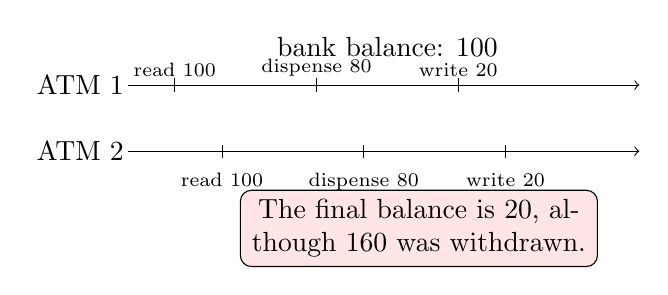
\begin{tikzpicture}[x=1cm,y=0.7cm]
  \node at (-0.6,0) {ATM 1};
  \node at (-0.6,-1.2) {ATM 2};
  \node at (3.3,0.7) {bank balance: $100$};
  \draw[->] (0,0) -- (6.5,0);
  \draw[->] (0,-1.2) -- (6.5,-1.2);
  \foreach \x/\lab in {0.6/read 100,2.4/dispense 80,4.2/write 20}
    \draw (\x,0.12) -- (\x,-0.12) node[above=2pt,font=\scriptsize] {\lab};
  \foreach \x/\lab in {1.2/read 100,3.0/dispense 80,4.8/write 20}
    \draw (\x,-1.08) -- (\x,-1.32) node[below=2pt,font=\scriptsize] {\lab};
  \node[draw,rounded corners,fill=red!10,text width=4.3cm,align=center] at (3.7,-2.6)
    {The final balance is $20$, although $160$ was withdrawn.};
\end{tikzpicture}
\end{center}
\visible<2->{
\begin{block}{Lesson}
Correctness may depend on all possible interleavings of concurrent actions.
\end{block}}
}
\end{frame}

\begin{frame}[fragile]{Three basic threats in parallel programming}
\Margines{
\begin{block}{Deadlock}
Consider philosophers following the protocol below.
\end{block}
\vspace{-0.15cm}
\DwieKol{0.46}{0.46}{
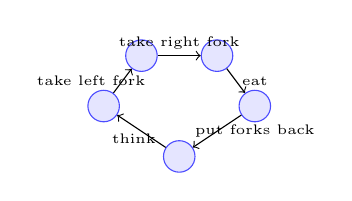
\begin{tikzpicture}[scale=0.32]
  \node[tinyState] (F1) at (3,0) {};
  \node[tinyState] (F2) at (0,2) {};
  \node[tinyState] (F3) at (1.5,4) {};
  \node[tinyState] (F4) at (4.5,4) {};
  \node[tinyState] (F5) at (6,2) {};
  \foreach \y/\x in {1/2,2/3,3/4,4/5,5/1}
      \draw[->] (F\y) -- (F\x);
   \node at (1.2,0.7) {\tiny think};
   \node at (6,1) {\tiny put forks back};
   \node at (-0.5,3) {\tiny take left fork};
   \node at (6,3) {\tiny eat};
   \node at (3,4.5) {\tiny take right fork};
\end{tikzpicture}
}{
\begin{center}
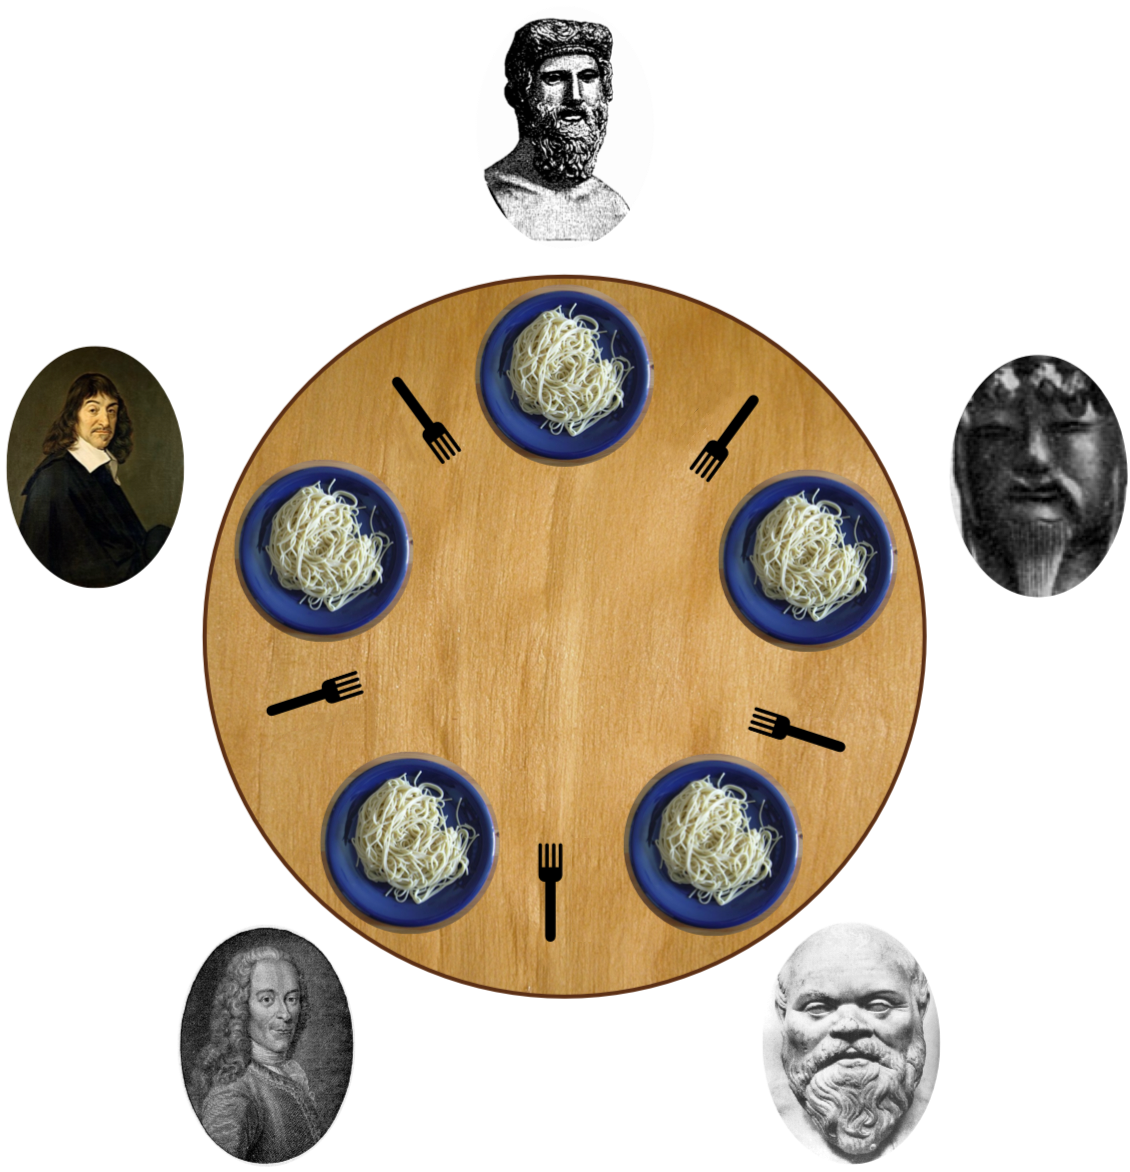
\includegraphics[width=0.38\linewidth]{5philo.png}
\end{center}
}
\vspace{-0.2cm}
\visible<2->{
\begin{block}{Deadlock scenario}
If all philosophers first take their left fork, then every philosopher waits for the right fork and no one can proceed.
\end{block}}
\visible<3->{
\begin{block}{Typical solution}
Break circular waiting, e.g. acquire forks according to a fixed global order.
\end{block}}
}
\end{frame}

\begin{frame}[fragile]{Three basic threats in parallel programming}
\Margines{
\begin{block}{Starvation}
A system may keep making progress while one process is repeatedly prevented from making progress.
\end{block}
\DwieKol{0.46}{0.46}{
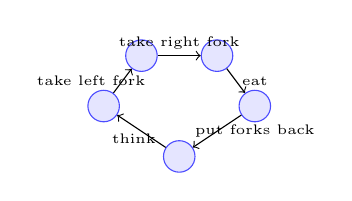
\begin{tikzpicture}[scale=0.32]
  \node[tinyState] (F1) at (3,0) {};
  \node[tinyState] (F2) at (0,2) {};
  \node[tinyState] (F3) at (1.5,4) {};
  \node[tinyState] (F4) at (4.5,4) {};
  \node[tinyState] (F5) at (6,2) {};
  \foreach \y/\x in {1/2,2/3,3/4,4/5,5/1}
      \draw[->] (F\y) -- (F\x);
   \node at (1.2,0.7) {\tiny think};
   \node at (6,1) {\tiny put forks back};
   \node at (-0.5,3) {\tiny take left fork};
   \node at (6,3) {\tiny eat};
   \node at (3,4.5) {\tiny take right fork};
\end{tikzpicture}
}{
\begin{center}
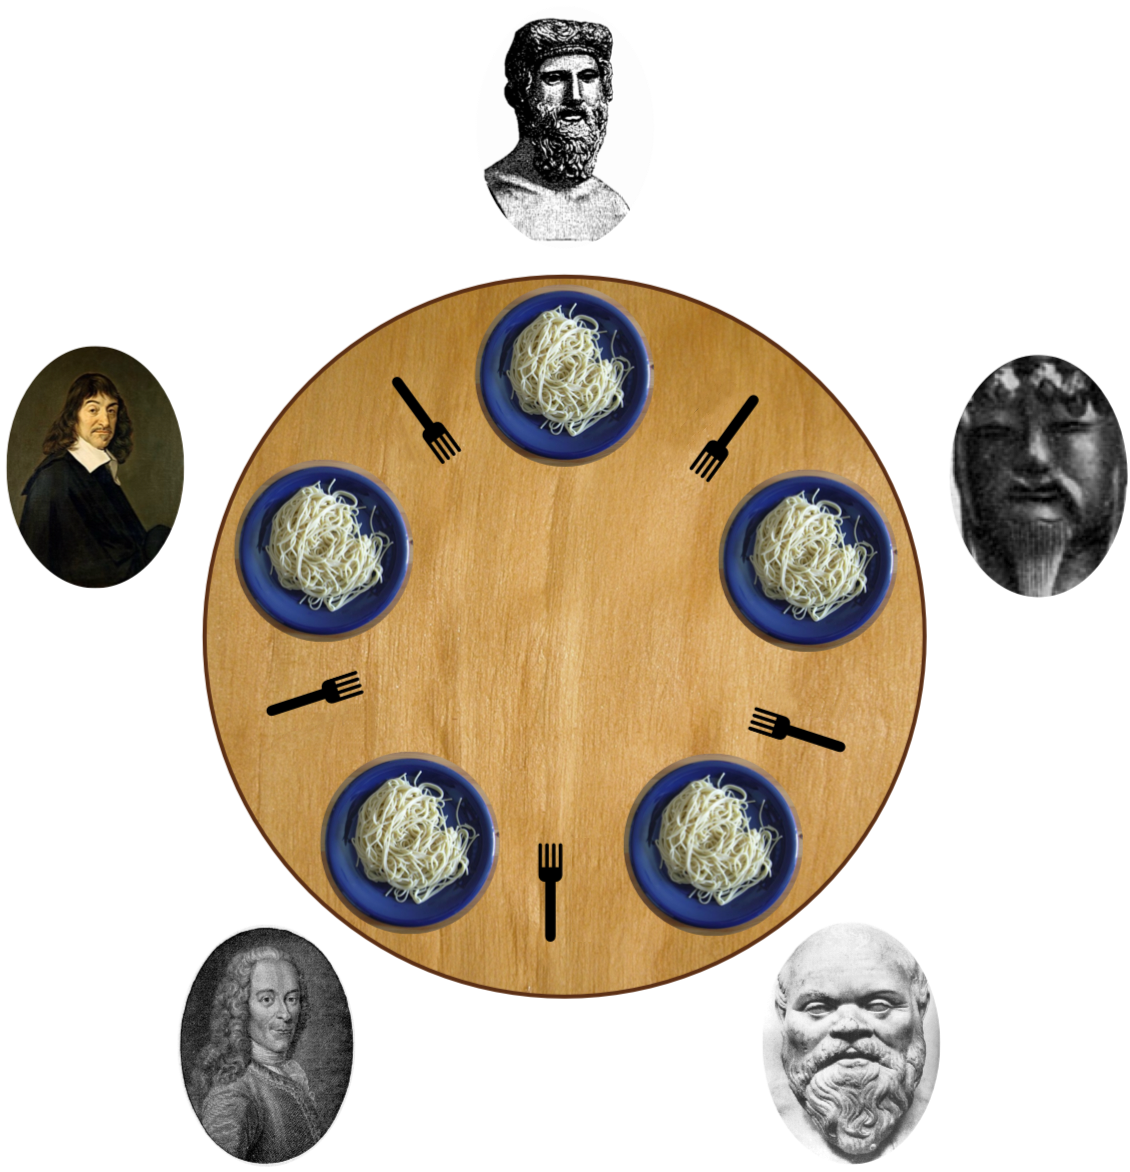
\includegraphics[width=0.38\linewidth]{5philo.png}
\end{center}
}
\vspace{-0.2cm}
\visible<2->{
\begin{block}{Typical solution}
Use a fair scheduling or allocation policy, e.g. FIFO access or bounded waiting.
\end{block}}
\visible<3->{
\begin{block}{Contrast with deadlock}
In a deadlock nobody progresses. Under starvation, the system progresses, but not fairly.
\end{block}}
}
\end{frame}

\begin{frame}{Goal of formal modelling}
\Margines{
\begin{block}{What we want}
We want mathematical models that describe all possible executions of a concurrent system and allow us to state which executions are correct.
\end{block}
\begin{itemize}
  \item Race condition: ``something bad never happens.''
  \item Deadlock freedom: ``the system can always make progress.''
  \item Starvation freedom: ``a process that keeps requesting access eventually succeeds.''
\end{itemize}
\visible<2->{
\begin{block}{Key difficulty}
The behaviour of a concurrent system is not one execution, but a set of possible executions.
\end{block}}
}
\end{frame}

\begin{frame}{How can we observe a running system?}
\Margines{
For now, we consider two simple forms of observation.
\begin{block}{Logs}
A running system records selected events as a log.
\end{block}
\begin{block}{Debugger}
A debugger allows us to inspect the system state step by step.
\end{block}
\begin{block}{Limitations}
\begin{itemize}
  \item Recording every event or every variable may be prohibitively expensive.
  \item Observing the system may itself change its behaviour, e.g. by affecting execution timing.
\end{itemize}
\end{block}
}
\end{frame}

\begin{frame}{Model}
\Margines{
\begin{block}{Model}
A model is a simplified representation of a system that preserves the aspects relevant to the question being studied.
\end{block}
\visible<2->{
\begin{block}{Abstraction}
We deliberately forget some information.
\begin{itemize}
  \item Logs expose only selected actions; other actions may be silent.
  \item State-based models expose only selected variables or predicates.
\end{itemize}
\end{block}}
\visible<3->{
\begin{block}{Consequence}
A proof about the model is meaningful only under the assumption that the model captures the relevant behaviour of the real system.
\end{block}}
}
\end{frame}

\begin{frame}{Kripke structures and labelled transition systems}
\Margines{
\begin{block}{General concept}
\begin{itemize}
  \item A system is always in some state, also called a configuration.
  \item The state may evolve during execution.
  \item States are vertices; possible evolutions are edges.
\end{itemize}
\end{block}
\DwieKol{0.47}{0.47}{
\mojBlock{0.95}{block}{Kripke structures}{
States are labelled by propositions that are true in the current state.
}}
{
\mojBlock{0.95}{block}{Labelled transition systems}{
Transitions are labelled by actions performed by the system.
}}
}
\end{frame}

\begin{frame}{Labelled transition systems}
\Margines{
\begin{block}{Definition}
A labelled transition system is a tuple
\[
T=(S,I,\Sigma,\rightarrow)
\]
where:
\begin{enumerate}
  \item $S$ is a set of states, possibly infinite;
  \item $I\subseteq S$ is a set of initial states;
  \item $\Sigma$ is a set of actions;
  \item $\rightarrow\subseteq S\times\Sigma\times S$ is a transition relation.
\end{enumerate}
We write $s\xrightarrow{a}s'$ for $(s,a,s')\in\rightarrow$.
\end{block}
\visible<2->{
\begin{block}{Runs and traces}
An infinite run is
\[
s_0\xrightarrow{a_0}s_1\xrightarrow{a_1}s_2\xrightarrow{a_2}\cdots
\]
where $s_0\in I$ and $s_i\xrightarrow{a_i}s_{i+1}$ for all $i\geq 0$.
Its trace is the infinite word $a_0a_1a_2\cdots\in \Sigma^\omega$.
\end{block}}
}
\end{frame}

\begin{frame}[fragile]{Example: simple communication protocol}
\Margines{
\begin{center}
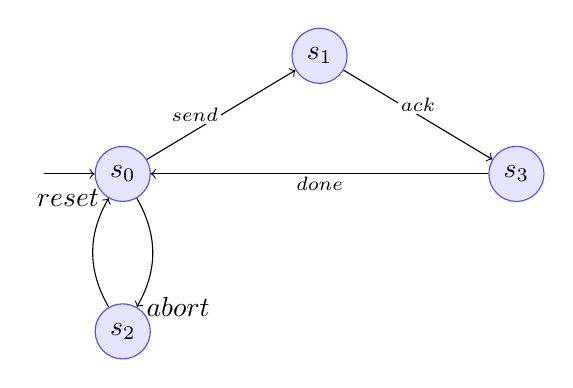
\begin{tikzpicture}
  \node[stateNode] (s0) at (0,0) {$s_0$};
  \node[stateNode] (s1) at (2.5,1.5) {$s_1$};
  \node[stateNode] (s2) at (0,-2) {$s_2$};
  \node[stateNode] (s3) at (5,0) {$s_3$};
  \draw[->] (-1,0) -- (s0);
  \draw[->] (s0) -- (s1) node[msg,left] {$send$};
  \draw[->] (s0) to[bend left] (s2) node[right] {$abort$};
  \draw[->] (s1) -- (s3) node[msg,above] {$ack$};
  \draw[->] (s2) to[bend left] (s0) node[left] {$reset$};
  \draw[->] (s3) -- (s0) node[msg,below] {$done$};
\end{tikzpicture}
\end{center}
\visible<2->{
\begin{itemize}
  \item Initial state: $s_0$.
  \item Actions: $\Sigma=\{send,ack,abort,reset,done\}$.
  \item Example infinite traces:
  \[
  (send\ ack\ done)^\omega
  \]
  and
  \[
  abort\ reset\ (send\ ack\ done)^\omega.
  \]
\end{itemize}}
}
\end{frame}

\begin{frame}{Kripke structures}
\Margines{
Let $\AProp$ be a set of atomic propositions.
\visible<2->{
\begin{block}{Definition}
A Kripke structure over $\AProp$ is a tuple
\[
M=(S,I,R,L)
\]
where:
\begin{enumerate}
  \item $S$ is a finite set of states;
  \item $I\subseteq S$ is a set of initial states;
  \item $R\subseteq S\times S$ is a left-total transition relation:
  \[
  \forall s\in S\ \exists s'\in S\quad (s,s')\in R;
  \]
  \item $L:S\to 2^{\AProp}$ labels each state by the propositions true in that state.
\end{enumerate}
\end{block}}
}
\end{frame}

\begin{frame}{Runs and traces of Kripke structures}
\Margines{
\begin{block}{Run}
An infinite run of a Kripke structure $M=(S,I,R,L)$ is a sequence
\[
s_0s_1s_2\cdots
\]
such that $s_0\in I$ and $(s_i,s_{i+1})\in R$ for every $i\geq 0$.
\end{block}
\visible<2->{
\begin{block}{Trace}
The trace of this run is
\[
L(s_0)L(s_1)L(s_2)\cdots\in (2^{\AProp})^\omega.
\]
The set of traces of all infinite runs of $M$ is denoted by $\trace{M}$.
\end{block}}
\visible<3->{
\begin{block}{Comparison}
LTS traces record actions. Kripke traces record properties of states.
\end{block}}
}
\end{frame}

\begin{frame}{Pros and cons of LTS and Kripke structures}
\Margines{
\begin{block}{Advantages}
\begin{itemize}
  \item They are simple and intuitive.
  \item They provide a precise operational model.
  \item They are useful for defining semantics of richer modelling formalisms.
\end{itemize}
\end{block}
\visible<2->{
\begin{block}{Limitations}
\begin{itemize}
  \item Explicit models may be very large.
  \item Large transition systems are difficult to inspect manually.
  \item They often hide the structural or modular description from which the state space was generated.
\end{itemize}
\end{block}}
\visible<3->{
For the first few lectures we will use them as basic models of systems.
}
}
\end{frame}

\begin{frame}{The language perspective}
\Margines{
\begin{block}{Idea}
A system model defines a language of possible behaviours. A specification can also be viewed as a language.
\end{block}
\visible<2->{
\begin{block}{Error language}
Let $E$ be the set of all erroneous behaviours. Then
\[
\trace{M}\cap E=\emptyset
\]
means that no behaviour of the system is erroneous.
\end{block}}
\visible<3->{
\begin{block}{Correct-behaviour language}
Let $P$ be the set of all acceptable behaviours. Then
\[
\trace{M}\subseteq P
\]
means that every behaviour of the system satisfies the specification.
\end{block}}
}
\end{frame}

\begin{frame}{Exercise: five philosophers}
\Margines{
\begin{block}{Modelling task}
\begin{itemize}
  \item Choose atomic propositions sufficient to describe the relevant behaviour.
  \item Describe the states and transitions of a corresponding Kripke structure.
  \item Draw a representative fragment of this Kripke structure.
\end{itemize}
\end{block}
\visible<2->{
\begin{block}{Properties to specify}
\begin{itemize}
  \item A philosopher can eat only while holding both forks.
  \item Every philosopher eats infinitely often.
  \item Rene Descartes eats infinitely often and thinks infinitely often.
\end{itemize}
\end{block}}
\visible<3->{
\begin{block}{Question}
How can these properties be specified over infinite traces?
\end{block}}
}
\end{frame}

\begin{frame}{Why infinite-word automata?}
\Margines{
\begin{block}{Reactive systems}
Concurrent and reactive systems may run forever. Their complete behaviours are naturally represented by infinite words.
\end{block}
\visible<2->{
\begin{block}{Finite automata are not enough}
Ordinary finite automata recognize languages of finite words. We need automata whose acceptance condition is defined for infinite runs.
\end{block}}
\visible<3->{
\begin{block}{Main question}
How should an automaton accept an infinite word?
\end{block}}
}
\end{frame}

\begin{frame}{Finite automata}
\Margines{
Let $\Sigma$ be a finite alphabet.
\begin{block}{Definition}
A nondeterministic finite automaton is a tuple
\[
A=(Q,\Sigma,I,F,\delta)
\]
where:
\begin{enumerate}
  \item $Q$ is a finite set of states;
  \item $I\subseteq Q$ is a set of initial states;
  \item $F\subseteq Q$ is a set of accepting states;
  \item $\delta\subseteq Q\times\Sigma\times Q$ is a transition relation.
\end{enumerate}
\end{block}
\visible<2->{
\begin{block}{Acceptance}
A finite word is accepted if it labels a path from an initial state to an accepting state.
\end{block}}
\visible<3->{
\begin{block}{Problem}
Our traces are infinite words.
\end{block}}
}
\end{frame}

\begin{frame}{Acceptance conditions for infinite words}
\Margines{
Let
\[
q_0\xrightarrow{a_0}q_1\xrightarrow{a_1}q_2\xrightarrow{a_2}\cdots
\]
be an infinite run.
\begin{itemize}
  \item<2-> Attempt 1: acceptance depends on some finite prefix.
  \item<3-> Attempt 2: from some point on, the run stays only in accepting states.
  \item<4-> Attempt 3: the run visits accepting states infinitely often.
  \item<5-> Attempt 4: the run visits each of several accepting sets infinitely often.
\end{itemize}
\visible<4->{
\begin{block}{B\"uchi idea}
Acceptance should express behaviour that occurs infinitely often.
\end{block}}
}
\end{frame}

\begin{frame}{\Buchi\ automata}
\Margines{
\begin{block}{Definition}
A \Buchi\ automaton is a tuple
\[
A=(Q,\Sigma,I,F,\delta)
\]
where $Q,\Sigma,I,\delta$ are as for a nondeterministic finite automaton, and $F\subseteq Q$ is the set of accepting states.
\end{block}
\visible<2->{
\begin{block}{Acceptance}
An infinite run
\[
q_0\xrightarrow{a_0}q_1\xrightarrow{a_1}q_2\xrightarrow{a_2}\cdots
\]
is accepting if it visits $F$ infinitely often:
\[
\{i\geq 0\mid q_i\in F\}\text{ is infinite.}
\]
\end{block}}
\visible<3->{
The language $\lang{A}$ is the set of infinite words that have an accepting run in $A$.
}
}
\end{frame}

\begin{frame}{Generalised \Buchi\ automata}
\Margines{
\begin{block}{Definition}
A generalised \Buchi\ automaton has several accepting sets
\[
\mathcal F=\{F_1,\ldots,F_k\},\qquad F_j\subseteq Q.
\]
\end{block}
\visible<2->{
\begin{block}{Acceptance}
An infinite run is accepting if it visits every accepting set infinitely often:
\[
\forall j\in\{1,\ldots,k\}\quad
\{i\geq 0\mid q_i\in F_j\}\text{ is infinite.}
\]
\end{block}}
\visible<3->{
\begin{block}{Example intuition}
This is useful for conjunctions of liveness requirements: each required event must happen infinitely often.
\end{block}}
}
\end{frame}

\begin{frame}{\Buchi\ languages}
\Margines{
\begin{block}{Lemma}
For every finite Kripke structure $M$ there is a \Buchi\ automaton $A$ such that
\[
\lang{A}=\trace{M}.
\]
\end{block}
\visible<2->{
\begin{block}{Lemma}
\Buchi\ and generalised \Buchi\ automata recognize the same class of languages.
\end{block}}
\visible<3->{
\begin{block}{\texorpdfstring{$\omega$}{omega}-regular languages}
Languages recognized by \Buchi\ automata are called \(\omega\)-regular languages. They are closed under union, intersection, and complement.
\end{block}}
\visible<4->{
\begin{block}{Determinisation warning}
Not every nondeterministic \Buchi\ automaton has an equivalent deterministic \Buchi\ automaton. Determinisation requires stronger acceptance conditions, e.g. parity acceptance.
\end{block}}
}
\end{frame}

\end{document}
